\subsection{Backend}

\subsubsection{Flask}
\begin{wrapfigure}{l}{0.5\textwidth}
    \centerline{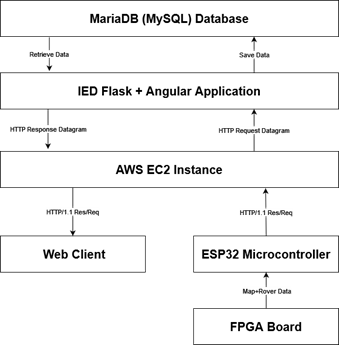
\includegraphics[width=0.45\textwidth]{images/backend-flow.png}}
    \caption{Backend design overview}
\end{wrapfigure}

The backend of the web application is based on Flask Web Framework. Flask is a lightweight framework used to build web applications using python \cite{ref:whatisflask}. Flask acts as the back-bone to the whole Tech stack providing the interfacing and connection between the frontend Angular application, The AWS EC2 instance and the MariaDB database.  

The choice of Flask was made primarily due to personal preference and due to prior experience with the Python programming language, Flask’s main advantage is its minimalistic design which allows for modularity and also, as it's written in Python, it enjoys the flexibility and extended support that the programming language allows for. The main reason why Flask was chosen instead of other technologies such as, JavaScript and Node.js is because of a steeper learning curve required in being able to build an entire web application~\cite{ref:nodevsflask} and it being more suited for a larger scale environment that is beyond the scope of this project.

The way the web application is designed out is thus: an AWS EC2 instance which holds the full stack application, the frontend in Angular and the backend in Flask which contains the ORM model of the database using a library called SQL-Alchemy, which allows for interfacing with MariaDB, a database based on the MySQL engine. This entire application is hosted on the AWS server, therefore the outside world will not be able to reach it normally. The application uses Gunicorn and NGINX to deal with that. Gunicorn is a Web Server Gateway Interface (WSGI)~\cite{ref:gunicorn} which allows for communication between the main Flask application and HTTP requests, it allows for Python to be able to understand and execute HTTP requests/responses, this is then paired with NGINX which is a web server that acts as a reverse proxy~\cite{ref:nginx} that allows requests sent to the AWS’ IP-address to be rerouted to your flask application. Using these technologies enable the linking of the web server and the web application including features that allow for reliability, maintainability, and scalability due to the services built-in both gunicorn and nginx. These services are what allow seamless integration of the RESTful API used and interfacing with the MariaDB instance.

\subsubsection{Database}
One of the functional requirements of the whole system is that the segway should store data about the map and about itself so that it can then be accessed, managed, and later retrieved. To do that a database is used for the project. MariaDB, a relational database running on the MySQL engine, was chosen as the database for the design. The choice was made by taking into consideration factors such as development time constraints, size of database and prior experience of the development team; MariaDB is chosen over vanilla MySQL due to its greater performance in speed when executing queries. 

The Relational Model consists of two primary entities, the Map, and the Segway. The Map is based on a typical graph data structure which uses vertices, “Nodes” and non-directional weighted edges. This implementation is used due to the requirement of being able to then calculate the shortest path and using a graph data structure allows us to then perform some sort of shortest path algorithm such as Dijkstra’s. The Segway entity’s main role is in providing the telemetry data to the front-end application, this includes data on the position of the segway, the accelerometer and gyroscope data and also data on the steps and date of the segway. This data is crucial in being able to locate the segway relative to the map and also provide the position of the nodes that make up the map, it also serves to assign the weights to each respective edge. 
\begin{wrapfigure}{l}{0.5\textwidth}
    \centerline{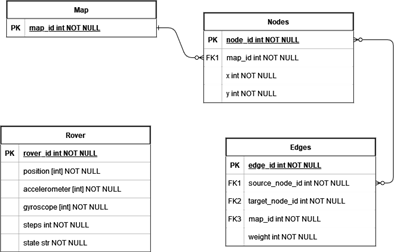
\includegraphics[width=0.45\textwidth]{images/map-orm.png}}
    \caption{Map relational model}
\end{wrapfigure}

Taking a closer look at the Map model, it will have an id which will then be used as a foreign key on the Node table, this establishes one to many relationship between the Map entity and the node entity, each map can have multiple nodes but not the other way round. In turn the Node table has its own identifier, values for the x and y coordinates and also the foreign key from the Map table. The Edge entity has multiple foreign keys, namely the ids of the source and target nodes, its own respective id and also a weighting parameter to keep track of the weight assigned to that particular edge, the Edge entity has a many to many relationship with the Node table as nodes can have multiple edges and edges attach to multiple nodes, the source and target node. It is important to assert these cardinality relationships as its what establishes the connections of the map and overall content that can then be retrieved by the server when either transmitting navigation commands or calculating the shortest path between the start and end nodes.

\subsubsection{REST API}
An API can be simply described as a set of protocols to be used as a universal method of communication between a client and a server~\cite{ref:restapi}. The API is an essential part of the Web server as it acts as a middleman between the web application and the segway it provides a way to organise and share resources and information whilst also providing security control and authentication. 
The main purpose of the API is to be able to display the front-end application when one enters the IP address of the AWS EC2 instance but also it is used as a way to perform CRUD operation. One example of this could be in the form of a POST request to send information to be stored to the database and conversely a GET request would return information particular to that request. One example of this would be sending the Telemetry data of the Segway, on the client side (the actual segway) data would be transmitted about he segway’s position, mpu6050 data and other necessary data, this would be done in the ESP32 microcontroller through a HTTP request, this request would contain in its body a JSON format file, the choice of using json was made due to its versatility and almost universal usage across various platforms.
For this specific use case there are currently seven routing endpoints in the API used. Three each for both the map and segway entities, and one for loading the index.html page. Taking a closer look at Telemetry for example when sending a POST request to update the segway’s data, the microcontroller would send a HTTP request to the server containing the necessary data, the server would receive it and route it to the API which would then perform the necessary functions and CRUD operation on the database.
